%% LyX 2.3.6 created this file.  For more info, see http://www.lyx.org/.
%% Do not edit unless you really know what you are doing.
\documentclass[english,aspectratio=169]{beamer}
\usepackage{lmodern}
\usepackage[inkscapelatex=false]{svg}
\renewcommand{\sfdefault}{lmss}
\renewcommand{\ttdefault}{lmtt}
\usepackage[T1]{fontenc}
\usepackage[latin9]{inputenc}
\setlength{\parskip}{\medskipamount}
\setlength{\parindent}{0pt}
\usepackage{babel}
\usepackage{array}
\usepackage{amssymb}
\usepackage{graphicx}
\PassOptionsToPackage{normalem}{ulem}
\usepackage{ulem}
\ifx\hypersetup\undefined
  \AtBeginDocument{%
    \hypersetup{unicode=true}
  }
\else
  \hypersetup{unicode=true}
\fi

\makeatletter

%%%%%%%%%%%%%%%%%%%%%%%%%%%%%% LyX specific LaTeX commands.
\pdfpageheight\paperheight
\pdfpagewidth\paperwidth

%% Because html converters don't know tabularnewline
\providecommand{\tabularnewline}{\\}

%%%%%%%%%%%%%%%%%%%%%%%%%%%%%% Textclass specific LaTeX commands.
% this default might be overridden by plain title style
\newcommand\makebeamertitle{\frame{\maketitle}}%
% (ERT) argument for the TOC
\AtBeginDocument{%
  \let\origtableofcontents=\tableofcontents
  \def\tableofcontents{\@ifnextchar[{\origtableofcontents}{\gobbletableofcontents}}
  \def\gobbletableofcontents#1{\origtableofcontents}
}

%%%%%%%%%%%%%%%%%%%%%%%%%%%%%% User specified LaTeX commands.
\usetheme{CambridgeUS}
%\usecolortheme{dove}
\hypersetup{pdfpagemode=None}
\usepackage{tikz}
\usepackage{color}
\usepackage{listings}

% This allows to change color of symbols in math
\newcommand*{\mathcolor}{}
\def\mathcolor#1#{\mathcoloraux{#1}}
\newcommand*{\mathcoloraux}[3]{%
  \protect\leavevmode
  \begingroup
    \color#1{#2}#3%
  \endgroup
}

\makeatother

\begin{document}
\title[Theory ]{Revision control}
\author{Marcello Vichi}
\institute[UCT]{Department of Oceanography\\marcello.vichi@uct.ac.za}
\date{AOS}
\makebeamertitle

\section*{Outlines}
\begin{frame}{Outline}

\tableofcontents{}

\begin{columns}[t]

\column{7cm}
\begin{itemize}
\item {\small{}You don't need to be a software engineer to appreciate the
importance of maintaining different revisions of various objects.
RCS have developed in the 80's for sequential and concurrent code
writing, but are now being expanded to handle multiple types of files}{\small\par}
\item {\small{}Revision Control is not just for BIG CODES (Source Code Management),
but also for routine activities, especially in a shared professional
environment}{\small\par}
\item {\small{}The material in this section is adapted from \href{http://swcarpentry.github.io/git-novice/}{http://swcarpentry.github.io/git-novice/}}{\small\par}
\end{itemize}

\column{7cm}


\includegraphics[scale=0.25]{figures/GIT-comic}
\end{columns}

\end{frame}
%
\begin{frame}{The concept}
\begin{columns}[t]

\column{8cm}
\begin{itemize}
\item {\footnotesize{}Revision control systems (RCS) start with a base version
of the document and then record changes you make each step of the
way. You can think of it as a recording of your progress: you can
rewind to start at the base document and play back each change you
made, eventually arriving at your more recent version}{\footnotesize\par}
\item {\footnotesize{}The terms }\textbf{\footnotesize{}version}{\footnotesize{}
and }\textbf{\footnotesize{}revision}{\footnotesize{} are often used
as synonyms. They have technical differences in software engineering.
A version is a more generic term to indicate changes in a file or
a set of files. Technically, it is often associated with }\textbf{\footnotesize{}releases}{\footnotesize{}
of a software or document (e.g. v1.2). Revision is any recorded change
or combination of changes.}{\footnotesize\par}
\end{itemize}
    
\column{5.5cm}
\begin{center}
\includesvg[width=0.75\columnwidth]{figures/play-changes.svg}
\par\end{center}
\begin{itemize}
\item {\small{}Once you think of changes as separate from the document itself,
you can then think about \textquotedblleft playing back\textquotedblright{}
different sets of changes on the base document, ultimately resulting
in different versions of that document.}{\small\par}
\end{itemize}
\end{columns}

\end{frame}
%
\begin{frame}{Concurrent versioning, committing and merging}
\begin{columns}[t]

\column{7cm}
\begin{center}
\includesvg[width=0.4\columnwidth]{figures/versions.svg}
\par\end{center}
\begin{itemize}
\item {\tiny{}Two users can make independent sets of changes on the same
document. This operation creates two }\textbf{\tiny{}concurrent}{\tiny{}
versions. A change to a file is a temporary modification in RCS: saving
the file is not sufficient to acknowledge the generation of a new
version. This further operation is called }\textbf{\tiny{}committing}{\tiny{}
a version}{\tiny\par}
\item {\tiny{}If the changes have been done to different parts, they are
}\textbf{\tiny{}complementary}{\tiny{}, and you can incorporate two
sets of changes into the same base document}{\tiny\par}
\item {\tiny{}If the changes have been done to the same section of the document
they generate a }\textbf{\tiny{}conflict}{\tiny{}. }{\tiny\par}
\end{itemize}

\column{7cm}
\begin{center}
\includesvg[width=0.4\columnwidth]{figures/merge.svg}
\par\end{center}
\begin{itemize}
\item {\tiny{}The operation of combining the different committed versions
is called }\textbf{\tiny{}merging}{\tiny{}. In the case of conflicts
it can be a very complicated process.}{\tiny\par}
\item {\tiny{}A RCS is a tool that keeps track of these changes for us,
effectively storing different versions of our files. It allows us
to decide which changes will be made to the next revision (each record
of these changes is called a }\textbf{\tiny{}commit}{\tiny{}), and
keeps useful metadata about them (when, who, what). }{\tiny\par}
\item {\tiny{}The complete history of commits for a particular project and
their metadata make up a }\textbf{\tiny{}repository}{\tiny{}. Repositories
can be }\textbf{\tiny{}distributed}{\tiny{}. They are kept in sync
across different computers (or your computer and a server in the cloud),
facilitating collaboration among different people.}{\tiny\par}
\end{itemize}
\end{columns}

\end{frame}
%
\begin{frame}{The GIT model: local and remote repositories}
\begin{columns}[t]

\column{6.5cm}

{\scriptsize{}GIT is now the most used RCS, thanks to its distributed
model. Git is a sophisticated software. It can get rather complex,
but the basic commands and procedures are quite simple }{\scriptsize\par}

{\footnotesize{}}%
\begin{tabular}{|>{\raggedright}p{1.5cm}|>{\raggedright}p{4cm}|}
\hline 
\textbf{\tiny{}Term} & \textbf{\tiny{}Meaning}\tabularnewline
\hline 
\hline 
{\tiny{}Workspace copy} & {\tiny{}Users' active directory. All files (including folders) in
this directory will be tracked}\tabularnewline
\hline 
{\tiny{}Stage Area} & {\tiny{}It is a place where all the modified files marked to be committed
are placed}\tabularnewline
\hline 
{\tiny{}Local Repository} & {\tiny{}User\textquoteright s copy of a remote repository. It must
be synchronized manually}\tabularnewline
\hline 
{\tiny{}Remote Repository} & {\tiny{}It is a server where all the collaborators upload changes
made to files}\tabularnewline
\hline 
{\tiny{}Clone Command} & {\tiny{}Creates a copy of an existing remote repository inside a local
repository}\tabularnewline
\hline 
\end{tabular}{\footnotesize\par}

\column{6cm}

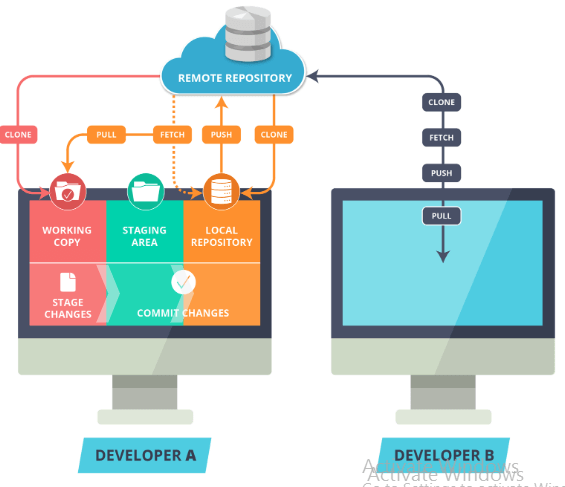
\includegraphics[width=4.5cm]{figures/Git-remote-local}
\begin{itemize}
\item {\tiny{}Commit: Commits all files from the staging area to local Repository}{\tiny\par}
\item {\tiny{}Push: Pushes all the changes made in local to Remote Repository}{\tiny\par}
\item {\tiny{}Fetch: Collects the changes from Remote Repository and copies
them to Local Repository but doesn't affect our workspace}{\tiny\par}
\item {\tiny{}Pull: Collects the changes from Remote Repository and copies
them to Local Repository along with merges to the current directory
or our workspace}{\tiny\par}
\end{itemize}
\end{columns}

\end{frame}
%
\begin{frame}{Public services: GitHub}
\begin{columns}[t]

\column{7cm}
\begin{itemize}
\item {\footnotesize{}\href{https://github.com}{GitHub} is a web-based
Git version control repository hosting service. It provides all of
the distributed version control and source code management functionalities
of Git for collaborative projects }{\footnotesize\par}
\item {\tiny{}Git}{\tiny\par}
\begin{itemize}
\item {\tiny{}It is a software }{\tiny\par}
\item {\tiny{}It is installed locally on the system }{\tiny\par}
\item {\tiny{}It is a tool to manage different versions of files}{\tiny\par}
\item {\tiny{}It is a command-line tool (some GUIs available but not recommended)}{\tiny\par}
\end{itemize}
\item {\tiny{}GitHub}{\tiny\par}
\begin{itemize}
\item {\tiny{}It is a service }{\tiny\par}
\item {\tiny{}It is hosted on the Web }{\tiny\par}
\item {\tiny{}It is a space to upload a copy of a Git repository }{\tiny\par}
\item {\tiny{}It provides a graphical interface through the browser }{\tiny\par}
\item {\tiny{}It enables to track issues and to create a collaborative development
environment}{\tiny\par}
\end{itemize}
\end{itemize}

\column{6cm}
\begin{center}
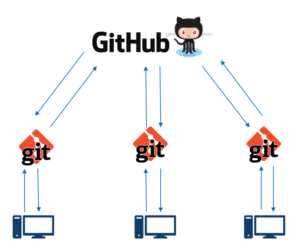
\includegraphics[scale=0.25]{figures/Github}
\par\end{center}
\begin{itemize}
\item {\scriptsize{}We will practice git using the tutorial on }{\scriptsize{}\uline{\href{http://swcarpentry.github.io/git-novice/}{Software Carpentry}}}{\scriptsize{}.
The practicals are in sections 1-9. The next sections are for information
on collaborative development}{\scriptsize\par}
\item {\scriptsize{}You are required to create an account on GitHub. \href{https://guides.github.com/activities/hello-world/}{https://guides.github.com/activities/hello-world/}}{\scriptsize\par}
\end{itemize}
\end{columns}

\end{frame}

\end{document}
